\section{Experiments}
\label{experiment}


\begin{figure*}[t]
  \centering
  \vspace{-4mm}
  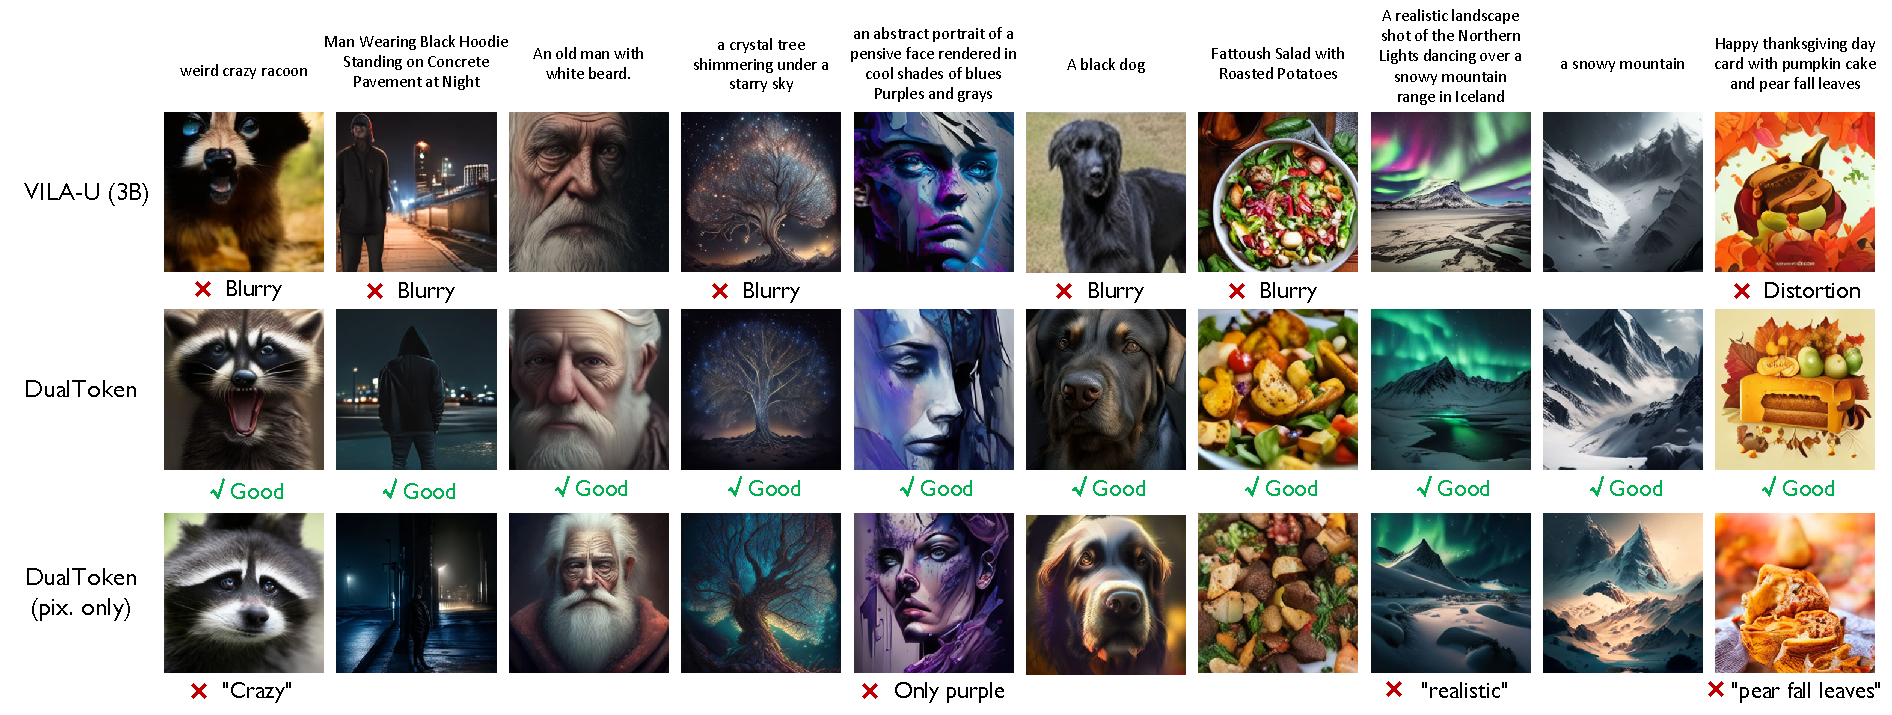
\includegraphics[width=\textwidth]{imgs/gen_cases-v4.pdf}
  \vspace{-4mm}
  \caption{Qualitative results on visual generation.}
  \label{fig:gen_cases}
  \vspace{-4mm}
\end{figure*}


\subsection{Vision Tokenizer}
\label{sec:exp_tokenizer}

\textbf{Experimental Setup~~} We trained two versions of our vision tokenizers at $256 \times 256$ and $384 \times 384$ resolutions. For fair comparison with VILA-U, we adopted the same quantization strategies and pretrained weights (SigLIP-L/16-256 and SigLIP-so/14-384), yielding 256 / 729 tokens with residual depths $D=4$ / $D=8$ (whereas VILA-U uses $D=4$ / $D=16$). To test stronger backbones, we further trained on SigLIP2-so/16-256 with $D=8$, and show that our method generalizes to other backbones in Appendix.~\ref{appendix_generalizability}. All models were trained on ImageNet-1K~\citep{deng2009imagenet}, CC12M~\citep{changpinyo2021cc12m}, and 50M images from LAION-400M~\citep{schuhmann2021laion400m}.

\textbf{Reconstruction~~} We measured reconstruction FID (rFID), PSNR, and SSIM on the ImageNet-1K (val). As shown in Table.\ref{tab:tokenizers}, our \ours{} achieves the highest structural similarity and the lowest rFID among various state-of-the-art dedicated methods, including Open-MAGVIT2 \citep{luo2024openmagvit2} and SBER-MoVQGAN \citep{sber2023movqgan}. This demonstrates that our method effectively mitigates the structural distortion and blurriness issues encountered by VILA-U during reconstruction.

\textbf{Semantic Metrics~~} For semantic metrics, we report the Top-1 accuracy for zero-shot classification on ImageNet-1K (val), along with text-to-image and image-to-text retrieval performance (R@1) on Flickr8K.
As shown in Table.\ref{tab:tokenizers}, our \ours{} significantly outperforms VILA-U and the latest concurrent work, UniTok, while also surpassing dedicated models like CLIP-L-14-336 in zero-shot image classification and achieves performance on par with the state-of-the-art SigLIP models.
%, without requiring any additional stages specifically designed to enhance semantic capabilities.
% We believe that incorporating an additional contrastive learning stage---where the shallow layers responsible for reconstruction are frozen while only the deeper layers are optimized for semantic objective---could further enhance the model's semantic performance.


\begin{table}[t]
  \centering
  \caption{\textbf{Controlled comparison across ten visual understanding benchmarks}. We evaluate different vision encoders/tokenizers, including siglip-large-16-256, VILA-U, and \ours{} within the LLaVA-1.5 framework. MMB refers to MMBench-dev~\citep{liu2023mmbench}, OCRB to OCRBench~\citep{liu2024ocrbench}, and TVQA to TextVQA~\citep{textvqa}. The MME~\citep{fu2024mme} score is normalized based on its total score. \textit{Sem.+Pix.} is the original setting of DualToken, where semantic and pixel tokens are concated along embedding dimension to serve as visual input. \textit{Sem. only} means only the semantic tokens are fed as visual input.}  
  \label{tab:llava}
  \resizebox{\linewidth}{!}{
  \tablestyle{3pt}{1.05}
  \begin{tabular}{ll|l|llllllllll|l}
  \toprule
   &Vision Encoder            &Res.&MMB                   & MME                       &SEED                  &VQAv2                &MMVet  &AI2D&MMMU&POPE                 & OCRB&TVQA &AVG.\\
  \midrule
   (a)&siglip-large-16-256  &$256$&60.9 & 62.9&56.4&78.2&34.5&53.5&30.8&80.3& 26.3& 44.3&52.8\\
  
   (b)&VILA-U                    &$256$&55.3\basenum{(-5.6)}& 53.8\basenum{(-9.1)}&51.2\basenum{(-5.6)}&73.1\basenum{(-5.1)}&24.9\basenum{(-9.6)}&49.4\basenum{(-4.1)}&28.4\basenum{(-2.4)}&78.2\basenum{(-2.1)}& 23.8\basenum{(-2.5)}& 42.8\basenum{(-1.5)}&48.1\basenum{(-4.7)}\\
  
   \compare{}(c)&\compare{}\ours{} (sem. only)     &\compare{}$256$&\compare{}59.8\loss{(-1.1)}& \compare{}63.0\gain{(+0.1)}&\compare{}56.2\loss{(-0.2)}&\compare{}77.6\loss{(-0.6)}&\compare{}34.0\loss{(-0.5)}&\compare{}53.7\gain{(+0.2)}&\compare{}30.3\loss{(-0.5)}&\compare{}79.4\loss{(-0.9)}&\compare{24.6}\loss{(-1.7)}&\compare{43.2}\loss{(-1.1)}&\compare{}52.2\loss{(-0.6)}\\
  
   \compare{}(d)&\compare{}\ours{} (sem.+ pix.)     &\compare{}$256$&\compare{}61.3\gain{(+0.4)}& \compare{}64.6\gain{(+1.7)}&\compare{}57.2\gain{(+0.8)}&\compare{}77.0\loss{(-1.2)}&\compare{}34.6\gain{(+0.1)}&\compare{}55.9\gain{(+2.4)}&\compare{}30.2\loss{(-0.6)}&\compare{}83.0\gain{(+2.7)}&\compare{}29.2\gain{(+2.9)}&\compare{}46.2\gain{(+1.9)}&\compare{53.9}\gain{(+1.1)}\\
  
  \bottomrule
  \end{tabular}
  }
  % \vspace{-8mm}
\end{table}


\textbf{Downstream Performance within LLaVA-1.5~~} Before formally introducing the performance of our unified model, we first conducted a controlled experiment to validate the effectiveness of our vision tokenizer in downstream MLLM understanding tasks within the LLaVA-1.5~\citep{liu2024llava1d5} framework. Specifically, we replace the vision encoder of LLaVA-1.5 with \ours{}, while strictly adhering to its training data and using LLaMA-2-7B~\citep{touvron2023llama} as the foundational LLM.
As shown in Table.\ref{tab:llava} \textcolor{purple}{(a)(b)(d)}, our \ours{}, as a discrete unified vision tokenizer, outperforms VILA-U and even surpasses the original continuous SigLIP model.


\subsection{Unified Model for Generation and Understanding}
\label{sec:exp_llm}

Building on the unified tokenizers, we further verified its potential within a unified AR framework based on Qwen-2.5-3B~\citep{yang2024qwen2d5}.
Our training process consists of four stages: (1) Freeze the LLM and pretrain on image-caption data, training only the visual projector for multimodal alignment. (2) Unfreeze the LLM and fine-tune on visual understanding data to enhance comprehension. (3) Freeze the LLM and train only the visual heads on text-to-image data. (4) Unfreeze all components and perform joint training on a mixture of understanding, generation, and interleaved datasets.

To ensure a fair comparison with VILA-U~\citep{wu2025vilau}, we additionally provide a reproduced version of VILA-U using Qwen-2.5-3B as the language backbone, trained with the same dataset and procedure as our method. % Please refer to Appendix.\ref{appendix_data} for the detailed dataset list. 
We evaluate our model against widely used vision-language understanding benchmarks, including VQAv2 \citep{vqa_v2}, POPE \citep{POPE}, MME \citep{fu2024mme}, SEED-IMG \citep{li2023seedbench}, MMBench \citep{liu2023mmbench}, and MM-Vet \citep{yu2023mmvet}. 
% For visual generation, we apply classifier-free guidance \citep{cfg} with a CFG value of 3.


\begin{table}[t!]
\setlength{\tabcolsep}{5.5pt}
\centering
\tablestyle{5pt}{1.1}
\caption{Quantitative results on visual understanding and generation benchmarks. }
\scalebox{0.69}{
    \begin{NiceTabular}{llcccccccc}
    \CodeBefore
    \Body
    \toprule
    Type         &Method                                    &\# Params  &POPE  &MMBench &SEED &MMMU  &MMVet &MathVista &MME\\
    \midrule
                 &InstructBLIP \citep{instructblip}         &7B             &-     &36.0    &58.8  &30.6 &26.2  &24.4      &1137.1\\
                 &LLaVA-Phi \citep{zhu2024llavaphi}         &2.7B           &85.0  &59.8    &-     &-    &28.9  &-         &1335.1\\
                 &LLaVA-1.5 \citep{liu2024llava1d5}         &7B             &85.9  &64.3    &58.6  &35.4 &31.1  &27.4      &1510.7\\
    \textit{Und.}&LLaVA-NeXT \citep{liu2024llavanext}       &7B             &86.5  &67.4    &70.2  &35.8 &43.9  &34.6      &1519.0\\
                 &\g{LLaVA-NeXT} \citep{liu2024llavanext}       &\g{34B}            &\g{87.7}  &{79.3}    &{75.9}  &\g{51.1} &\g{57.4}  &\g{46.5}      &\g{1631.0}\\
                 &ShareGPT4V \citep{chen2024sharegpt4v}     &7B             &-     &68.8    &69.7  &37.2 &37.6  &26.5      &1567.4\\
                 &VILA \citep{lin2024vila}                  &7B             &85.5  &68.9    &61.1  &-    &34.9  &-         &1533.0\\
    \midrule
                 &\g{BAGAL} \citep{bagel}                   &\g{14B}        &\g{-}  &\g{85.0}    &\g{-}  &\g{55.3} &\g{67.2}  &\g{73.1}      &\g{1687.0}\\
                 % &DreamLLM \citep{dong2024dreamllm}         &7B             &-     &58.2    &-     &-    &36.6  &-         &-\\
                 % &SEEDLLaMA \citep{ge2023seedllama}         &7B             &-     &45.8    &51.5  &-    &-     &-         &-\\
                 &Chameleon \citep{team2024chameleon}       &7B             &-     &31.1    &-     &22.4 &8.3   &-         &-\\
                 &Emu3 \citep{wang2024emu3}                 &8B             &85.2  &58.5    &68.2  &31.6 &-     &-         &-\\
                 &Show-o \citep{xie2024showo}               &1.5B           &73.8  &-       &-     &25.1 &-     &-         &948.4\\
                 &Janus \citep{wu2024janus}                 &1.5B           &87.0  &69.4    &63.7  &30.5 &34.3  &-         &1338.0\\
                 &Liquid \citep{liquid}                     &7B             &83.2  &-       &-     &-    &-     &-         &1448.0\\
                 &MUSE-VL (256px) \citep{xie2025musevl}     &7B             &-     &72.1    &69.1  &39.7 &-     &51.3      &1480.9\\
                 % &TokenFlow (256px) \citep{qu2024tokenflow} &13B            &85.0  &60.3    &62.6  &34.4 &27.7  &-         &1365.4\\
    \textit{Uni.}&TokenFlow (384px) \citep{qu2024tokenflow} &13B            &86.8  &68.9    &68.7  &38.7 &40.7  &-         &1545.9\\
                 % &TokLIP (384px) \citep{lin2025toklip}      &7B             &84.9  &76.9    &71.5  &47.1 &-     &-         &1496.6\\
                 &UniTok (256px) \citep{unitok}             &7B             &83.2  &61.1    &-     &-    &33.9  &-         &1448.0\\
                 &UniToken (384px) \citep{jiao2025unitoken} &7B             &-     &71.1    &69.9  &32.8 &-     &38.5      &-\\
                 &Show-o2 (432px) \citep{xie2025showo2}     &1.5B           &-     &67.4    &65.6  &37.1 &-     &-         &1450.9\\
                 &Show-o2 (432px) \citep{xie2025showo2}     &7B             &-     &79.3    &69.8  &48.9 &-     &-         &1620.5\\
                 &VILA-U \citep{wu2025vilau}                &7B             &85.8  &-       &59.0  &-    &33.5  &-         &1401.8\\
    \compare{}&\compare{}\ours{}-3B (256px) &\compare{}3B   &\compare{}86.0 &\compare{}70.9 &\compare{}70.2 &\compare{}38.6 &\compare{}32.5 &\compare{}46.5 &\compare{}1489.2\\
    \compare{}&\compare{}\ours{}-3B (384px) &\compare{}3B   &\compare{}88.1 &\compare{}76.2 &\compare{}72.2 &\compare{}40.3 &\compare{}40.2 &\compare{}49.2 &\compare{}1588.4\\
    \compare{}&\compare{}\ours{}-7B (256px) &\compare{}7B   &\compare{}88.6 &\compare{}74.9 &\compare{}71.8 &\compare{}45.8 &\compare{}40.5 &\compare{}55.8 &\compare{}1502.7\\
    \compare{}&\compare{}\ours{}-7B (384px) &\compare{}7B   &\compare{}89.4 &\compare{}80.0 &\compare{}72.5 &\compare{}47.4 &\compare{}44.3 &\compare{}57.6 &\compare{}1625.0\\
    \bottomrule
    \end{NiceTabular}}\\
    \vspace{1mm}
    (a) Evaluation on multimodal understanding benchmarks. \\
    \vspace{1mm}
\scalebox{0.72}{
    \begin{NiceTabular}{clccccccc}
    \CodeBefore
    \Body
    \toprule
    \multirow{2}{*}{{Type}} &\multirow{2}{*}{{Method}} & \multirow{2}{*}{{Architecture}} & 
    \multirow{2}{*}{Count{$\uparrow$}} & \multirow{2}{*}{Differ{$\uparrow$}} & \multirow{2}{*}{Compare{$\uparrow$}} & \multicolumn{2}{c}{Logical{$\uparrow$}} & \multirow{2}{*}{Overall{$\uparrow$}}   \\
    \cmidrule{7-8}
    &  &  & & &  & Negate & Universal   \\
    \midrule
    % &SD v2.1 \citep{latentdiffusion} & Diffusion & 0.68 & 0.70 & 0.68 & 0.54 & 0.64 & 0.62 \\
    &SD-XL \citep{sdxl} & Diffusion & 0.71 & 0.73 & 0.69 & 0.50 & 0.66 & 0.63 \\
    \textit{Gen.} &Midjourney v6 \citep{midjourney} & Diffusion & 0.78 & 0.78 & 0.79 & 0.50 & 0.76 & 0.69 \\
    &DALL-E 3 \citep{dalle3} & Diffusion & 0.82 & 0.78 & 0.82 & 0.48 & 0.80 & 0.70 \\
    \midrule
    &Show-o \citep{xie2024showo} & Discrete Diff. & 0.70  & 0.62 & 0.71 & 0.51 & 0.65 & 0.60 \\
    &ILLUME \citep{wang2024illume} & AR+Diff. & 0.66  & 0.68 &  0.67 & 0.49 & 0.63 & 0.60 \\
    &LWM \citep{lwm} & Autoregressive & 0.59 & 0.58 & 0.54 & 0.49 & 0.52 & 0.53 \\
    &Liquid~\citep{liquid} & Autoregressive & 0.76 & 0.73 & 0.74 & 0.46 & 0.74 & 0.65 \\
    \textit{Uni.} &UniTok~\citep{unitok} & Autoregressive & 0.76 & 0.76 & 0.79 & 0.46 & 0.73 & 0.67 \\
    &VILA-U~\citep{wu2025vilau} & Autoregressive & 0.70 & 0.71 & 0.74 & 0.53 & 0.66 & 0.64 \\
    \compare{}&\compare{}VILA-U 3B (256) & \compare{}Autoregressive & \compare{}0.68 & \compare{}0.66 & \compare{}0.70 & \compare{}0.49 & \compare{}0.64 & \compare{}0.60 \\
    \compare{}&\compare{}DualToken-3B (256) & \compare{}Autoregressive & \compare{}0.76 & \compare{}0.76 & \compare{}0.78 & \compare{}0.50 & \compare{}0.72 & \compare{}0.68 \\
    \midrule
    \baseline{}&\baseline{}DualToken-3B (pix. only) &\baseline{}Autoregressive & \baseline{}0.59 &\baseline{}0.59 &\baseline{}0.59 &\baseline{}0.47 & \baseline{}0.59 &\baseline{}0.55 \\
    \bottomrule
    \end{NiceTabular}} \\
    \vspace{1mm}
     (b) VQAScores on \textit{advanced} prompts of GenAI-Bench~\citep{GenAI-Bench}
    \vspace{-10pt}
\label{tab:main}
\end{table}


As shown in Table.\ref{tab:main}, our \ours{} (3B) demonstrates strong understanding performance compared to other unified models and surpasses dedicated understanding models like LLaVA-NeXT and ShareGPT4V~\citep{chen2024sharegpt4v}.
Meanwhile, as illustrated in Fig.~\ref{fig:gen_cases}, thanks to the significantly improved reconstruction quality of \ours{}, the generated images are rich in detail and structurally realistic, accurately capturing fine textures such as animal fur and other intricate patterns---effectively resolving the blurriness and distortions observed in VILA-U.
What’s more, the generated images exhibit remarkable alignment with the text, even for long and complex prompts. This is especially evident when compared with the \textit{pix. only} method (which only predicts pixel tokens during image generation), as it often ignores important semantic content during generation---highlighting the crucial role that semantic tokens play in helping the model grasp the semantic structure of images throughout the generation process. Results on more generation benchmarks are presented in Appendix.\ref{appendix_genbench}.

Beyond its impressive performance, we observed two interesting findings:
\begin{itemize}[leftmargin=*]
    \item \emph{Pixel tokens enhance understanding.} As shown in Table.\ref{tab:llava}~\textcolor{purple}{(a)(c)(d)}, we compared using only the semantic tokens (sem.), and a combination of semantic and pixel tokens (sem.+pcpt), concatenated along the embedding dimension to serve as visual input. Surprisingly, compared to using semantic tokens alone, jointly leveraging both semantic and pixel tokens leads to consistent improvements across various aspects, including general VQA~\citep{liu2023mmbench,fu2024mme}, hallucination detection~\citep{POPE}, and OCR-related benchmarks~\citep{textvqa,liu2024ocrbench}. Suggesting that the supplementation of high-frequency details by pixel tokens can compensate for the subtle semantic loss introduced by vector quantization.
    \item \emph{Semantic tokens also helps to generate.} As shown in Fig.\ref{fig:gen_cases} and Table.\ref{tab:main} \textcolor{purple}{(b)}, incorporating semantic tokens into the model’s autoregressive generation process leads to more semantically aligned image generation compared to using visual appearance tokens alone. This indicates that visual semantic tokens—beyond their role in understanding tasks—can also assist the model in grasping the semantic composition of images, thereby producing outputs that better align with the intended semantics. This is also clearly reflected in the model’s performance on GenAI-Bench.
\end{itemize}

\textbf{DualToken versus dual-encoder.} Recently, some studies have adopted dual-encoder designs to obtain visual representations~\citep{huang2025illume+}. Specifically, a VQVAE-based pixel encoder and a CLIP-based semantic encoder. To address a fundamental question---why is it necessary to obtain dual visual vocabularies within a unified tokenizer rather than simply combining existing specialized encoders? we conducted an experiment using the codebook from SBER-MoVQGAN as the low-level vocabulary and a VQ-processed SigLIP as the high-level vocabulary, as illustrated in Fig.\ref{fig:frameworks}~\textcolor{purple}{(a)}.

\begin{minipage}[h]{0.33\textwidth}
    As shown in Table.\ref{tab:mjhq}, this straightforward approach leads to significantly inferior image generation performance (See Appendix.\ref{implement} for implementation details). To explain this discrepancy, we visualize the feature spaces of DualToken’s 6th and 26th layers, as well as those of MoVQGAN and SigLIP with UMAP (Fig.\ref{tab:umap}).
\end{minipage}
\hfill
\begin{minipage}[h]{0.35\textwidth}
\vspace{-0.05cm}
    \centering
    \captionsetup{type=table}
    \caption{Results on the MJHQ-30K dataset~\citep{playground}.}
    \vspace{-0.1cm}
    \tablestyle{5pt}{1.16}
    \resizebox{0.96\linewidth}{!}{
        \begin{tabular}{lcccc}
        \toprule 
        Method & Type & Res. & FID$\downarrow$ \\
        \midrule
        SD-XL \citep{sdxl} & Diffusion & 1024 & 9.55 \\
        PixArt \citep{pixart} & Diffusion & 1024 & 6.14 \\ 
        Playground \citep{playground} & Diffusion & 1024 & 4.48 \\
        Liquid \citep{liquid} & Autoregressive & 512 & 5.47 \\
        Janus \citep{wu2024janus} & Autoregressive & 384 & 10.10 \\
        LWM \citep{lwm} & Autoregressive & 256 & 17.77 \\
        Show-o \citep{xie2024showo} & Discrete Diff. & 256 & 15.18 \\
        VILA-U 7B \citep{wu2025vilau} & Autoregressive & 256 & 12.81 \\
        \midrule
        \compare{}VILA-U 3B & \compare{}Autoregressive & \compare{}256 & \compare{}15.12 \\
        \compare{}DualToken 3B & \compare{}Autoregressive & \compare{}256 & \compare{}7.88 \\
        \midrule
        \compare{}\textit{Dual Encoder} & \compare{}Autoregressive & \compare{}256 & \compare{}17.55 \\
        \bottomrule
        \end{tabular}
    }
    % \vspace{-2mm}
    \label{tab:mjhq}
\end{minipage}
\hfill
\begin{minipage}[h]{0.283\textwidth}
    \centering
    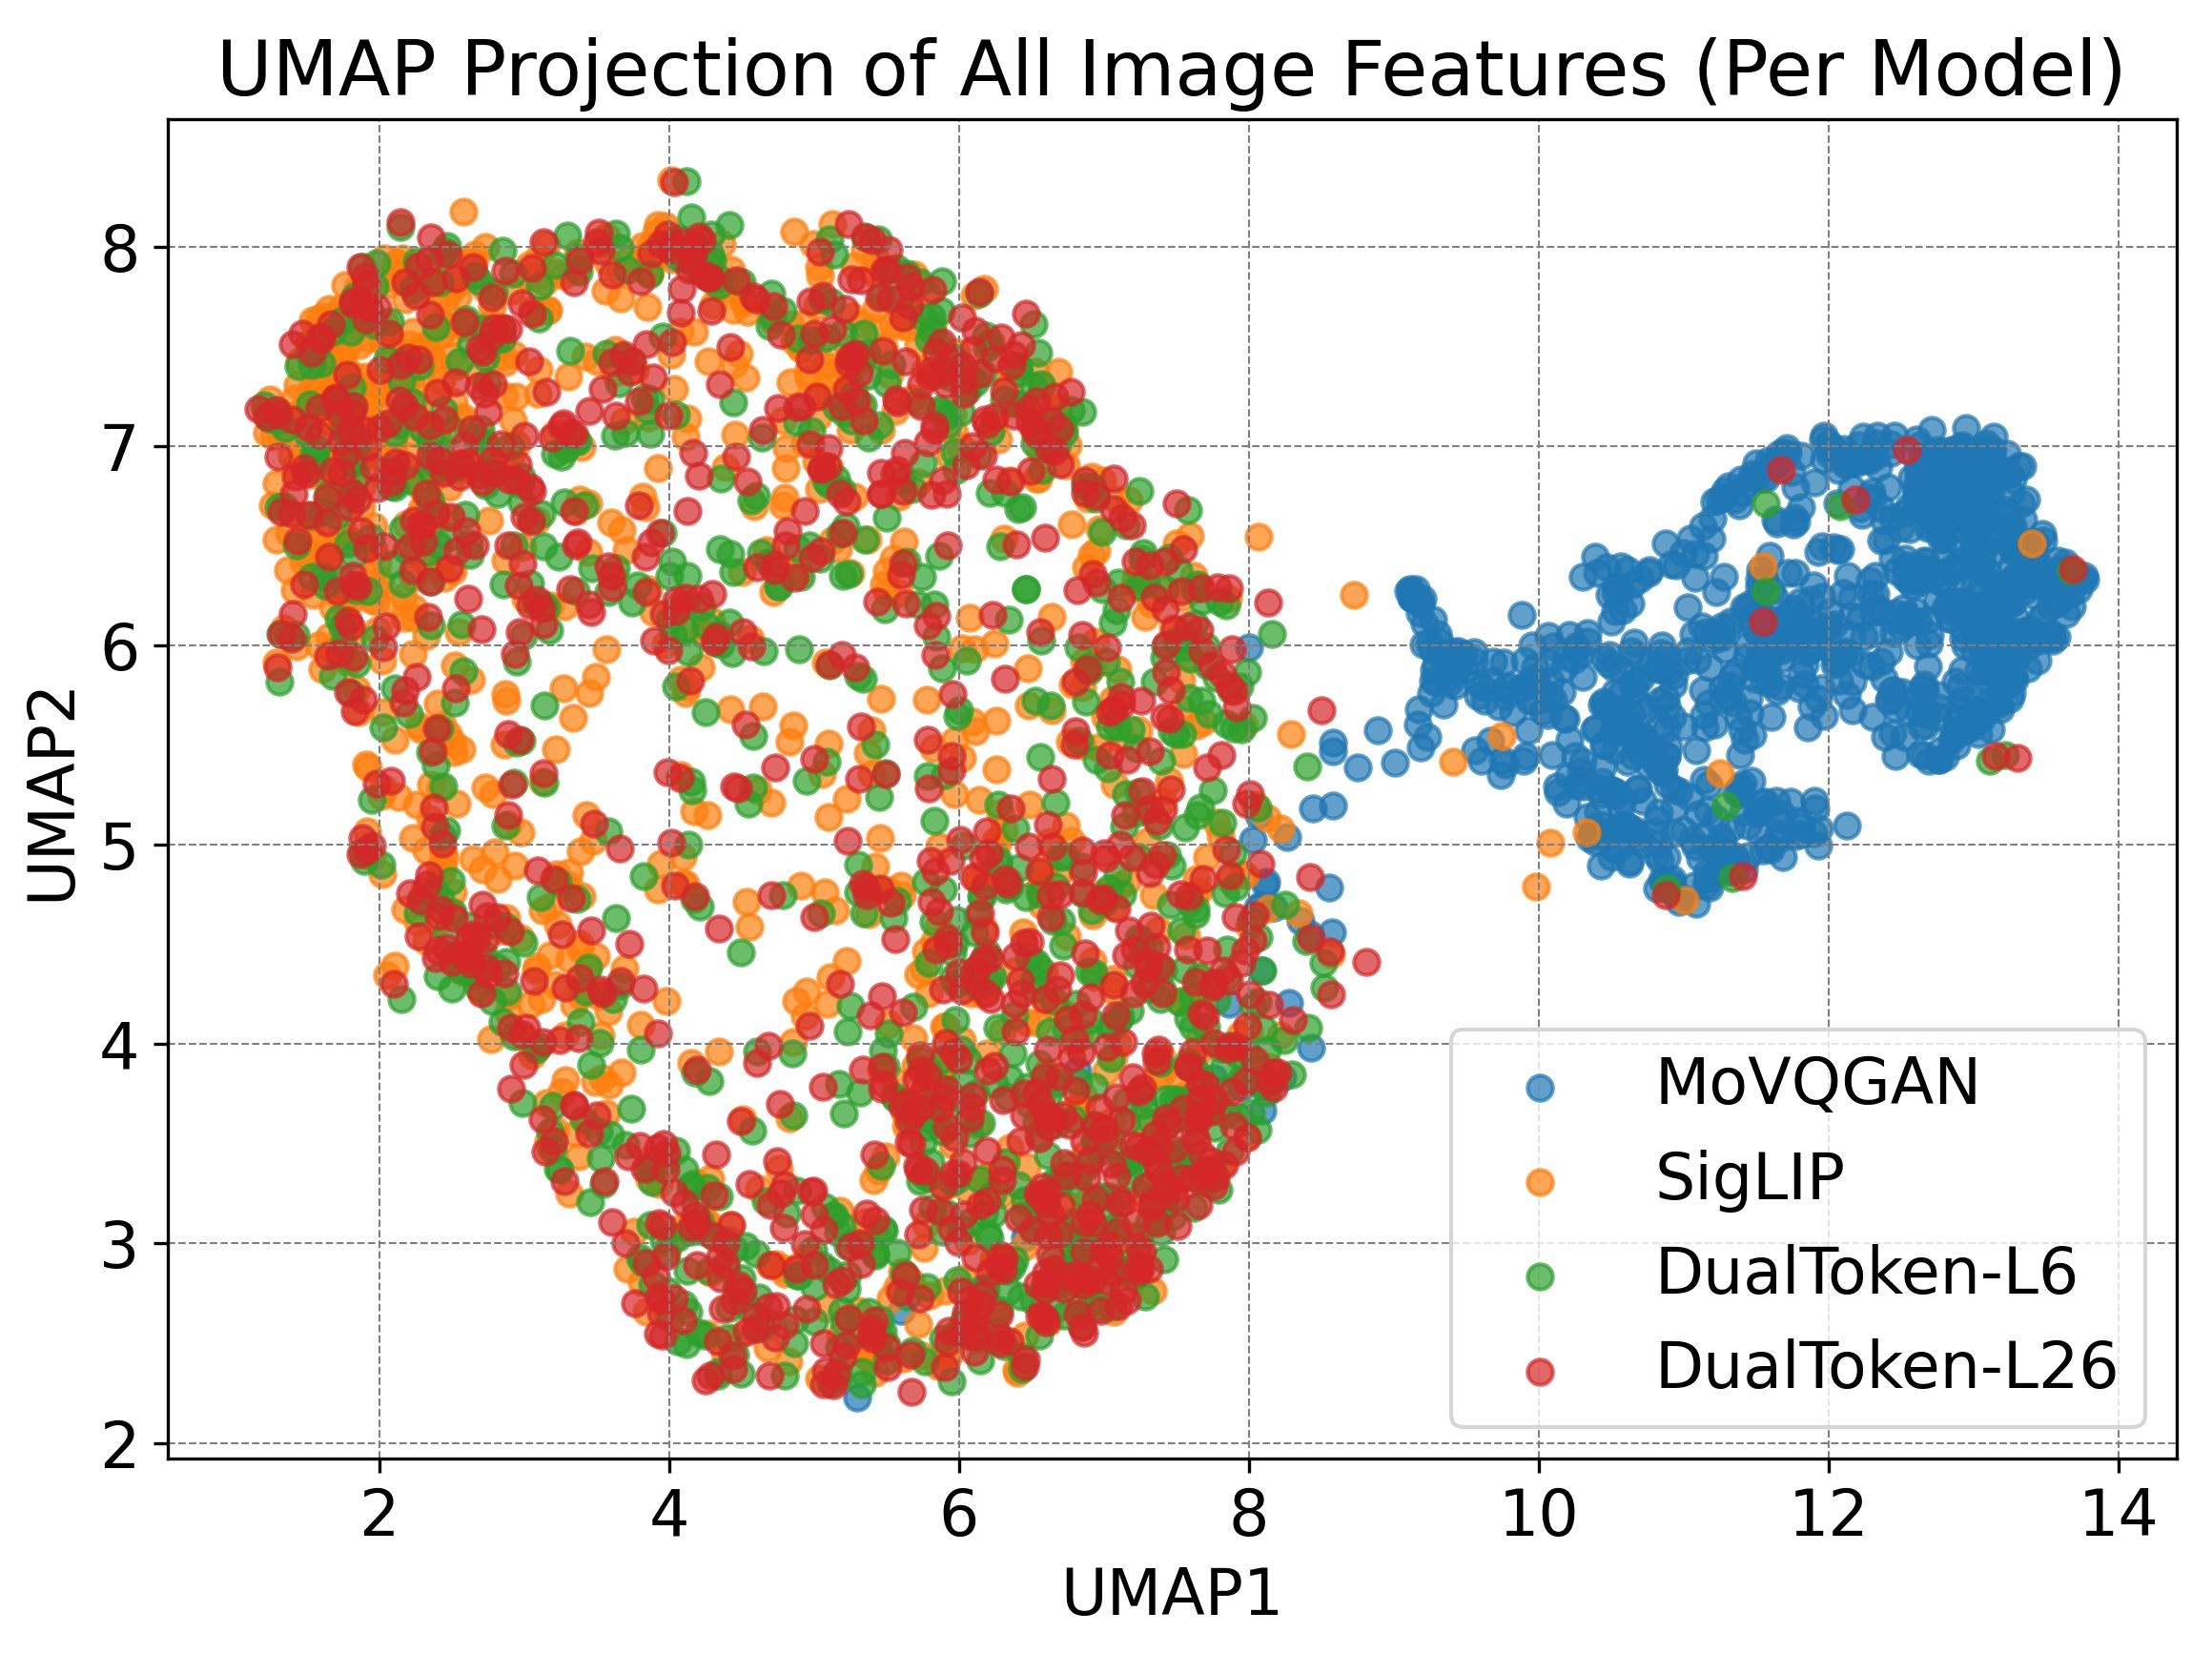
\includegraphics[height=2.95cm]{imgs/umap.png}

    \vspace{-0.15cm}
    
    \captionsetup{type=figure}
    \caption{Visualized feature spaces on Imagenet-1k (val).}
    \label{tab:umap}
\end{minipage}

As shown, while DualToken’s 6th and 26th layers yield features specialized for different purposes, they still share a largely overlapping representational space. In contrast, features from the two separate encoders (MoVQGAN and SigLIP) show significant divergence, forming clearly disjoint clusters.
Therefore, we attribute the performance gap to the incompatibility of representational spaces between heterogeneous encoders. This mismatch imposes a burden on the downstream language model, which is forced to learn two entirely disjoint visual representation systems. This observation further highlights the simplicity and effectiveness of DualToken as a unified architectural solution.

% ==== 平均特征之间的距离计算结果 ====
% [Group 1] MoVQGAN vs SigLIP:
%     L2 Distance:     12.5902
%     Cosine Distance: 1.4060
% [Group 2] DualToken Layer 6 vs Layer 26:
%     L2 Distance:     1.5961
%     Cosine Distance: 0.0675

% ==== 图像级特征距离的平均值 ====
% [Group 1] MoVQGAN vs SigLIP:
%     Average L2 Distance:     22.9014
%     Average Cosine Distance: 1.0425
% [Group 2] DualToken Layer 6 vs Layer 26:
%     Average L2 Distance:     2.2314
%     Average Cosine Distance: 0.0178